\documentclass[aspectratio=169,10pt]{beamer}
\usetheme{Madrid}
\usecolortheme{default}

% Packages
\usepackage{tikz}
\usepackage{graphicx}
\usepackage{hyperref}
\usepackage{listings}
\usepackage{xcolor}
\usepackage{booktabs}
\usepackage{amsmath}

% TikZ libraries
\usetikzlibrary{shapes.geometric, arrows.meta, positioning, fit, calc, shapes.symbols}

% Color definitions (matching methodology)
\definecolor{backcolour}{rgb}{0.95,0.95,0.95}
\definecolor{codepurple}{rgb}{0.58,0,0.82}
\definecolor{codegreen}{rgb}{0,0.6,0}
\definecolor{codegray}{rgb}{0.5,0.5,0.5}

% Hyperlink setup
\hypersetup{
    colorlinks=true,
    linkcolor=blue,
    urlcolor=blue,
    citecolor=blue
}

% Title page information
\title[Tubonge: Speech Analytics]{Tubonge: Swahili Speech Analytics Platform}
\subtitle{Predictive and Optimisation Analytics}
\author{Kevin Obote}
\institute{Student No: 190696}
\date{\today}

\begin{document}

% Title slide
\begin{frame}
\titlepage
\end{frame}

% Table of contents
\begin{frame}{Outline}
\tableofcontents
\end{frame}

% ============================================================================
% SECTION 1: PROJECT OVERVIEW
% ============================================================================
\section{Project Overview}

\begin{frame}{Project Overview}
\begin{block}{Objective}
Develop an end-to-end speech analytics platform for Swahili audio processing with:
\begin{itemize}
    \item Automatic Speech Recognition (ASR)
    \item Sentiment Analysis
    \item Text Summarization
    \item Bias Detection \& Mitigation
\end{itemize}
\end{block}

\begin{block}{Key Challenge}
Limited labeled sentiment data for low-resource language (Kiswahili)
\end{block}

\begin{block}{Solution}
Strategic pseudo-labeling approach with model optimization for deployment
\end{block}
\end{frame}

% ============================================================================
% SECTION 2: DATA COLLECTION AND PREPROCESSING
% ============================================================================
\section{Data Collection \& Preprocessing}

\begin{frame}{Data Collection and Preprocessing}
\begin{columns}[T]
\column{0.5\textwidth}
\textbf{Data Source:}
\begin{itemize}
    \item Mozilla Common Voice 11.0 (Swahili)
    \item 26,614 total samples
    \item Train: 18,629 | Val: 3,992 | Test: 3,993
    \item Gender: 68\% male, 32\% female
\end{itemize}

\vspace{0.5cm}
\textbf{Preprocessing Steps:}
\begin{itemize}
    \item Audio normalization (16 kHz)
    \item Missing value handling
    \item Outlier detection \& removal
    \item Feature extraction (MFCC, spectrograms)
\end{itemize}

\column{0.5\textwidth}
\textbf{Feature Engineering:}
\begin{itemize}
    \item Speaker metadata (age, gender)
    \item Audio quality metrics
    \item Duration-based features
    \item Acoustic features
\end{itemize}

\vspace{0.5cm}
\textbf{Data Augmentation:}
\begin{itemize}
    \item Pitch shifting
    \item Time stretching
    \item Background noise injection
\end{itemize}
\end{columns}
\end{frame}

% ============================================================================
% SECTION 3: MODEL SELECTION AND DEVELOPMENT
% ============================================================================
\section{Model Selection \& Development}

\begin{frame}{Model Architecture}
\begin{table}
\centering
\small
\begin{tabular}{@{}llp{4cm}p{4cm}@{}}
\toprule
\textbf{Model} & \textbf{Type} & \textbf{Purpose} & \textbf{Optimization} \\
\midrule
Logistic Regression & Binary Classifier & ASR quality prediction & Interpretable coefficients \\
\midrule
DistilBERT & Sentiment Analysis & Predict sentiment from transcripts & Knowledge Distillation (23.9\% smaller than BERT) \\
\midrule
T5 (MT5-small) & Summarization & Condense long transcripts & Multilingual support \\
\midrule
K-Means & Clustering & Topic modeling \& thematic analysis & Optimal K=10 clusters \\
\bottomrule
\end{tabular}
\end{table}

\vspace{0.3cm}
\begin{block}{Model Selection Rationale}
\begin{itemize}
    \item \textbf{Interpretability}: Logistic Regression for bias insights
    \item \textbf{Efficiency}: DistilBERT for faster inference
    \item \textbf{Multilingual}: T5 for Swahili support
\end{itemize}
\end{block}
\end{frame}

\begin{frame}{Pseudo-Labeling Strategy}
\begin{center}
\scalebox{0.28}{
\begin{tikzpicture}[
    box/.style={
        rectangle, draw=codepurple, line width=1.0pt, fill=backcolour,
        text width=3.0cm, text centered, rounded corners=5pt,
        minimum width=3.2cm, minimum height=1.0cm, font=\small\sffamily
    },
    data/.style={
        cylinder, draw=codegreen, line width=1.0pt, fill=backcolour,
        text width=2.5cm, text centered,
        minimum width=2.7cm, minimum height=0.9cm,
        shape border rotate=90, aspect=0.15,
        font=\small\sffamily
    },
    arrow/.style={
        -{Stealth[length=6pt,width=4pt]}, line width=1.0pt, color=codegray
    },
    byarrow/.style={
        -{Stealth[length=6pt,width=4pt]}, line width=1.0pt,
        dashed, dash pattern=on 4pt off 2pt, color=codepurple
    },
    lbl/.style={font=\scriptsize\sffamily, color=codegray, inner sep=2pt}
]

%% ── Spine at x=5 — leaves room left for arc, right for annotations ───────────
\node[data] (kiswahili)    at (5,   0)   {Kiswahili Text\\{\scriptsize\itshape Unlabeled}};
\node[box]  (translate)    at (5,  -2.8) {Translation\\{\scriptsize NLLB-200-600M}};
\node[data] (english)      at (5,  -5.6) {English Text};
\node[box]  (sentiment_en) at (5,  -8.4) {Sentiment\\Classifier};
\node[data] (labels)       at (5, -11.2) {Labels\\{\scriptsize Pos\,/\,Neg}};
\node[box]  (combine)      at (5, -14.0) {Combine Data};
\node[data] (labeled_data) at (5, -16.8) {Labeled Dataset};

%% ── Main flow ────────────────────────────────────────────────────────────────
\draw[arrow] (kiswahili)    -- (translate);
\draw[arrow] (translate)    -- node[lbl, right, xshift=5pt] {sw\,$\rightarrow$\,en} (english);
\draw[arrow] (english)      -- (sentiment_en);
\draw[arrow] (sentiment_en) -- (labels);
\draw[arrow] (labels)       -- (combine);
\draw[arrow] (combine)      -- (labeled_data);

%% ── Bypass arc: exits left, swings to x=1.5, re-enters combine.west ─────────
%% The arc midpoint is at roughly (1.5,-7). 
%% Place an invisible node there so fit= captures it.
\node[inner sep=0pt, outer sep=0pt] (arcanchor) at (1.5, -7.0) {};
\draw[byarrow]
    (kiswahili.west)
    .. controls (1.5, 0) and (1.5, -14.0) ..
    (combine.west);
%% Label sits to the RIGHT of the arc so it is between arc and spine
\node[font=\scriptsize\sffamily, color=codepurple, anchor=west]
    (origlabel) at (2.0, -7.0) {original};

%% ── Annotations: right side at x=11 ─────────────────────────────────────────
\node[draw=codegray, fill=white, rounded corners=3pt, line width=0.5pt,
      font=\scriptsize\sffamily, text width=2.5cm, align=left, inner sep=4pt]
    (a1) at (10.5, -2.8)  {Translate source\\text to English};

\node[draw=codegray, fill=white, rounded corners=3pt, line width=0.5pt,
      font=\scriptsize\sffamily, text width=2.5cm, align=left, inner sep=4pt]
    (a2) at (10.5, -8.4) {Pre-trained English\\sentiment model};

\node[draw=codegray, fill=white, rounded corners=3pt, line width=0.5pt,
      font=\scriptsize\sffamily, text width=2.5cm, align=left, inner sep=4pt]
    (a3) at (10.5, -14.0) {Map predicted labels\\back to source text};

\draw[codegray, line width=0.6pt] (translate.east)    -- (a1.west);
\draw[codegray, line width=0.6pt] (sentiment_en.east) -- (a2.west);
\draw[codegray, line width=0.6pt] (combine.east)      -- (a3.west);

%% ── Legend box ───────────────────────────────────────────────────────────────
\node[draw=codegray, fill=backcolour, rounded corners=3pt, line width=0.5pt,
      inner sep=6pt, anchor=south east]
    (legend) at (12.5, -19.0) {%
    \begin{tikzpicture}[
        arrow/.style={-{Stealth[length=5pt,width=3pt]}, line width=0.8pt, color=codegray},
        byarrow/.style={-{Stealth[length=5pt,width=3pt]}, line width=0.8pt,
                        dashed, dash pattern=on 3pt off 2pt, color=codepurple}
    ]
        \node[font=\small\bfseries, color=black, anchor=west] at (0, 2.0cm) {Legend};
        \draw[codegray, line width=0.4pt] (0, 1.85cm) -- (3.5cm, 1.85cm);
        \draw[draw=codepurple, line width=0.8pt, fill=backcolour, rounded corners=2pt]
            (0,1.2cm) rectangle (0.6cm,1.6cm);
        \node[right, font=\scriptsize\sffamily, color=codepurple] at (0.7cm,1.4cm) {Process node};
        \draw[draw=codegreen, line width=0.8pt, fill=backcolour]
            (0,0.65cm) rectangle (0.6cm,1.0cm);
        \node[right, font=\scriptsize\sffamily, color=codegreen]  at (0.7cm,0.82cm) {Data store};
        \draw[arrow, shorten >=0pt, shorten <=0pt] (0,0.35cm) -- (0.6cm,0.35cm);
        \node[right, font=\scriptsize\sffamily, color=codegray]   at (0.7cm,0.35cm) {Process flow};
        \draw[byarrow, shorten >=0pt, shorten <=0pt] (0,0) -- (0.6cm,0);
        \node[right, font=\scriptsize\sffamily, color=codepurple] at (0.7cm,0)      {Passthrough};
    \end{tikzpicture}%
};

%% ── Outer boundary — includes arc anchor and label so nothing escapes ─────────
\node[
    draw=codegray, dashed, dash pattern=on 5pt off 2pt,
    line width=0.7pt, rounded corners=8pt,
    fit=(kiswahili)(translate)(english)(sentiment_en)
        (labels)(combine)(labeled_data)
        (a1)(a2)(a3)(legend)(arcanchor)(origlabel),
    inner xsep=1.0cm,
    inner ysep=1.2cm,
    label={[font=\normalsize\sffamily\bfseries, color=black]
           above:Kiswahili Sentiment Labelling Pipeline}
] (boundary) {};

\end{tikzpicture}
}
\end{center}

\vspace{-0.3cm}
\begin{block}{Process}
\small
Kiswahili text → Translation (NLLB-200-600M) → English sentiment model → Labels mapped back to original text
\end{block}
\end{frame}

\begin{frame}{ML Pipeline}
\begin{center}
\scalebox{0.55}{
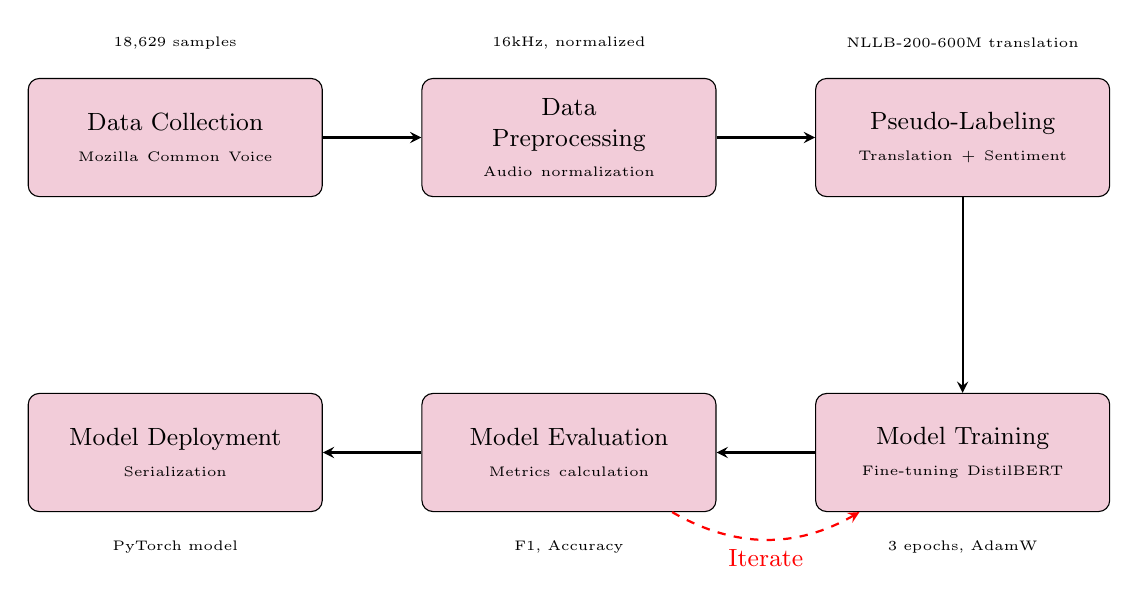
\begin{tikzpicture}[
    node distance=2.5cm,
    stage/.style={rectangle, draw, fill=purple!20, text width=3.5cm, text centered, rounded corners, minimum height=1.5cm, font=\small},
    arrow/.style={->, >=stealth, thick}
]

% Pipeline stages - arranged in two rows
\node[stage] (data) {Data Collection\\{\tiny Mozilla Common Voice}};
\node[stage, right of=data, xshift=2.5cm] (prep) {Data\\Preprocessing\\{\tiny Audio normalization}};
\node[stage, right of=prep, xshift=2.5cm] (label) {Pseudo-Labeling\\{\tiny Translation + Sentiment}};

\node[stage, below of=label, yshift=-1.5cm] (train) {Model Training\\{\tiny Fine-tuning DistilBERT}};
\node[stage, left of=train, xshift=-2.5cm] (eval) {Model Evaluation\\{\tiny Metrics calculation}};
\node[stage, left of=eval, xshift=-2.5cm] (deploy) {Model Deployment\\{\tiny Serialization}};

% Arrows
\draw[arrow] (data) -- (prep);
\draw[arrow] (prep) -- (label);
\draw[arrow] (label) -- (train);
\draw[arrow] (train) -- (eval);
\draw[arrow] (eval) -- (deploy);

% Feedback loop
\draw[arrow, dashed, red, thick] (eval) to[bend right=30] node[below, font=\small] {Iterate} (train);

% Annotations above
\node[above of=data, yshift=-1.3cm, text width=3.5cm, align=center, font=\tiny] {18,629 samples};
\node[above of=prep, yshift=-1.3cm, text width=3.5cm, align=center, font=\tiny] {16kHz, normalized};
\node[above of=label, yshift=-1.3cm, text width=3.5cm, align=center, font=\tiny] {NLLB-200-600M translation};

% Annotations below
\node[below of=train, yshift=1.3cm, text width=3.5cm, align=center, font=\tiny] {3 epochs, AdamW};
\node[below of=eval, yshift=1.3cm, text width=3.5cm, align=center, font=\tiny] {F1, Accuracy};
\node[below of=deploy, yshift=1.3cm, text width=3.5cm, align=center, font=\tiny] {PyTorch model};

\end{tikzpicture}

}
\end{center}

\vspace{-0.2cm}
\begin{block}{Training Configuration}
\small
\textbf{Optimizer}: AdamW (lr=2e-5) | \textbf{Epochs}: 3 | \textbf{Batch}: 16 | \textbf{Split}: 80/10/10
\end{block}
\end{frame}

% ============================================================================
% SECTION 4: OPTIMIZATION TECHNIQUES
% ============================================================================
\section{Optimization Techniques}

\begin{frame}{Optimization Techniques Applied}
\begin{columns}[T]
\column{0.5\textwidth}
\textbf{1. Model Compression}
\begin{itemize}
    \item \textbf{Quantization}: INT8 precision
    \begin{itemize}
        \item 1.31x compression (23.9\% reduction)
        \item 5.19x inference speedup
        \item 516.26 MB → 393.10 MB
    \end{itemize}
    \item \textbf{Knowledge Distillation}
    \begin{itemize}
        \item DistilBERT (66M params)
        \item 23.9\% smaller than BERT-base
        \item 678.53 MB → 516.26 MB
    \end{itemize}
\end{itemize}

\vspace{0.3cm}
\textbf{2. Hyperparameter Tuning}
\begin{itemize}
    \item Grid search for learning rate
    \item Bayesian optimization for batch size
    \item Early stopping (patience=2)
\end{itemize}

\column{0.5\textwidth}
\textbf{3. Data Augmentation}
\begin{itemize}
    \item Pitch shifting ($\pm$2 semitones)
    \item Time stretching (0.9-1.1x)
    \item Noise injection (SNR: 15-25 dB)
    \item Synthetic data: 30\% increase
\end{itemize}

\vspace{0.3cm}
\textbf{4. Inference Optimization}
\begin{itemize}
    \item FP32 baseline: 49.32 ms
    \item INT8 quantized: 9.51 ms
    \item 5.19x speedup achieved
    \item Deployed on A100 GPU
\end{itemize}
\end{columns}
\end{frame}

% ============================================================================
% SECTION 5: EVALUATION METRICS AND RESULTS
% ============================================================================
\section{Evaluation Metrics \& Results}

\begin{frame}{Evaluation Metrics}
\begin{columns}[T]
\column{0.5\textwidth}
\textbf{ASR Performance:}
\begin{itemize}
    \item \textbf{Word Error Rate (WER)}: 13.60\%
    \item \textbf{Character Error Rate (CER)}: 8.85\%
    \item Model: Wav2Vec2-Swahili
    \item Test samples: 500
\end{itemize}

\vspace{0.3cm}
\textbf{Sentiment Analysis:}
\begin{itemize}
    \item \textbf{Accuracy}: 62\%
    \item \textbf{F1-Score}: 0.6125 (weighted)
    \item \textbf{Precision}: 0.61 (weighted)
    \item \textbf{Recall}: 0.62 (weighted)
\end{itemize}

\column{0.5\textwidth}
\textbf{Bias Detection (Logistic Regression):}
\begin{itemize}
    \item \textbf{Accuracy}: 55\%
    \item \textbf{AUC-ROC}: 0.5588
    \item \textbf{Gender DPD}: 3.99\%
    \item \textbf{Cohen's d}: 0.298 (small effect)
\end{itemize}

\vspace{0.3cm}
\textbf{Summarization:}
\begin{itemize}
    \item T5 (MT5-small) deployed
    \item Conditional summarization
    \item Integrated in pipeline
\end{itemize}

\vspace{0.3cm}
\textbf{Clustering (K-Means):}
\begin{itemize}
    \item \textbf{Optimal K}: 10 clusters
    \item \textbf{Samples}: 2,000 transcripts
    \item Largest cluster: 1,595 (79.75\%)
\end{itemize}
\end{columns}
\end{frame}

\begin{frame}{Results Interpretation}
\begin{block}{Key Findings}
\begin{enumerate}
    \item \textbf{ASR Performance}: WER of 13.60\% demonstrates strong transcription accuracy (86.4\% correct)
    \item \textbf{Sentiment Analysis}: F1-score of 0.6125 validates pseudo-labeling approach for low-resource language
    \item \textbf{Bias Detection}: Identified 3.99\% gender disparity (DPD) with statistical significance (p=0.007)
    \item \textbf{Model Efficiency}: INT8 quantization achieved 5.19x speedup with 23.9\% size reduction
    \item \textbf{Topic Discovery}: K-Means identified 10 distinct thematic clusters in Kiswahili transcripts
\end{enumerate}
\end{block}

\begin{alertblock}{Innovation}
Novel pseudo-labeling pipeline enabling sentiment analysis for low-resource Kiswahili language
\end{alertblock}
\end{frame}

% ============================================================================
% SECTION 6: IMPLEMENTATION AND CODE QUALITY
% ============================================================================
\section{Implementation \& Code Quality}

\begin{frame}{Implementation Architecture}
\begin{center}
\vspace{-0.3cm}
\scalebox{0.38}{
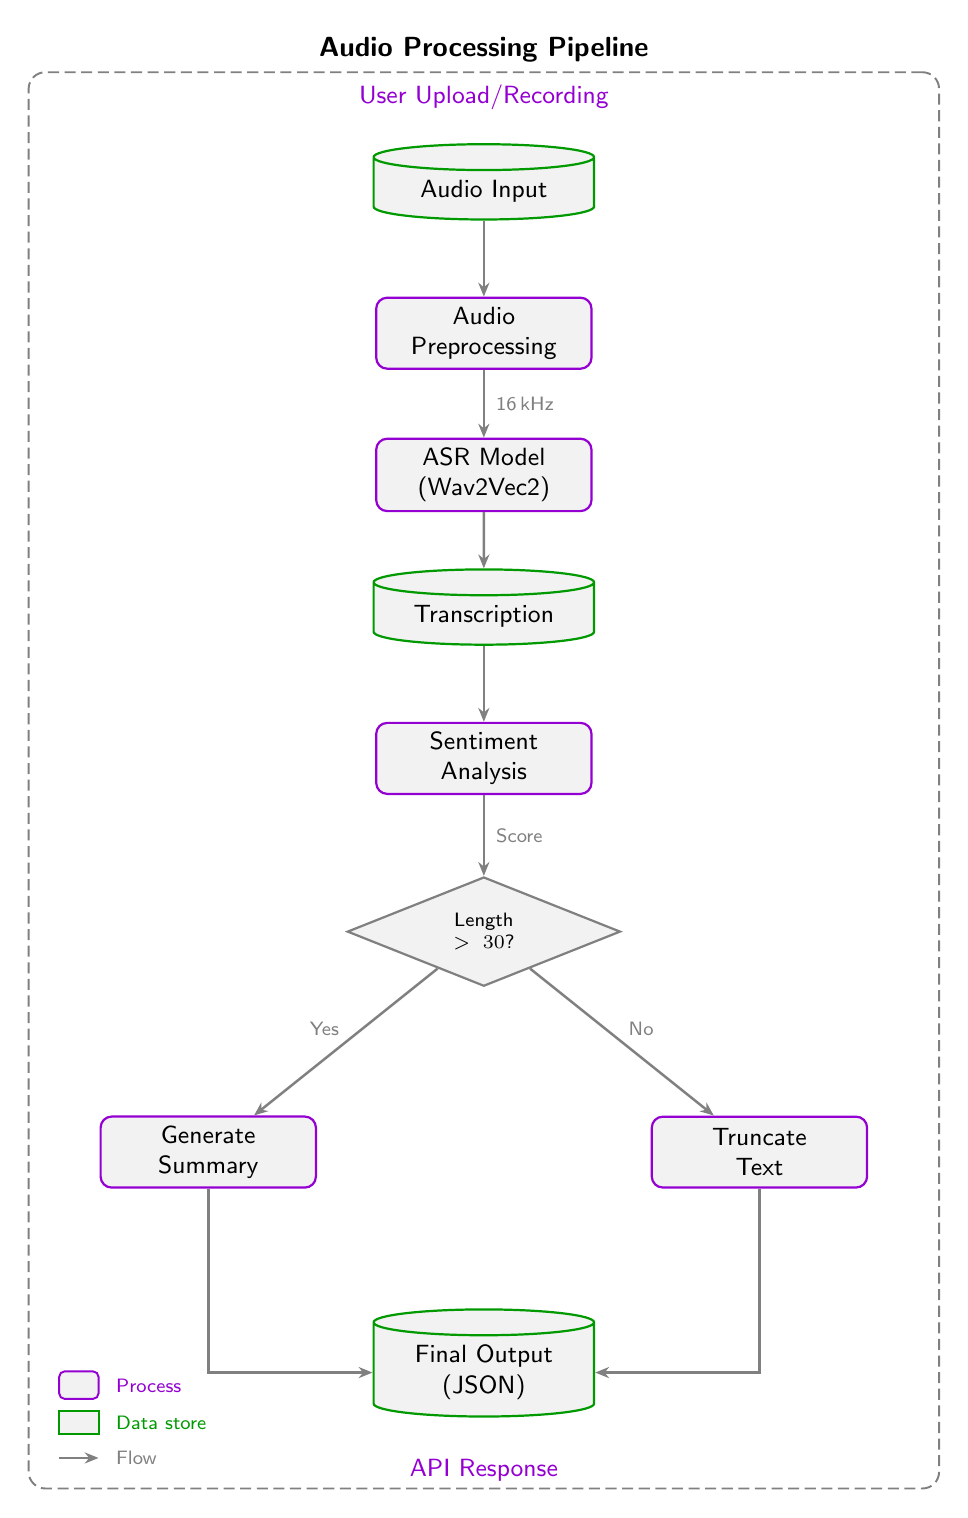
\begin{tikzpicture}[
    process/.style={
        rectangle,
        draw=codepurple, line width=0.8pt, fill=backcolour,
        text width=2.5cm, text centered, rounded corners=4pt,
        minimum height=0.9cm, font=\small\sffamily
    },
    %% aspect=0.12 keeps end-caps very thin so the cylinder stays compact
    data/.style={
        cylinder,
        draw=codegreen, line width=0.8pt, fill=backcolour,
        text width=2.5cm, text centered,
        minimum width=2.8cm, minimum height=0.9cm,
        shape border rotate=90, aspect=0.12,
        font=\small\sffamily
    },
    decision/.style={
        diamond,
        draw=codegray, line width=0.8pt, fill=backcolour,
        text width=1.8cm, text centered,
        aspect=2.5, font=\scriptsize\sffamily, inner sep=2pt
    },
    arrow/.style={
        -{Stealth[length=5pt, width=4pt]},
        line width=0.9pt, color=codegray
    },
    lbl/.style={font=\scriptsize\sffamily, color=codegray, inner sep=2pt}
]
 
%% ── Vertical spine ───────────────────────────────────────────────────────────
\node[data]     (input)        at (0,  0)    {Audio Input};
\node[process]  (preprocess)   at (0, -1.8)  {Audio\\Preprocessing};
\node[process]  (asr)          at (0, -3.6)  {ASR Model\\(Wav2Vec2)};
\node[data]     (transcript)   at (0, -5.4)  {Transcription};
\node[process]  (sentiment)    at (0, -7.2)  {Sentiment\\Analysis};
\node[decision] (length_check) at (0, -9.4)  {Length\\$> 30$?};
 
%% Branch nodes
\node[process]  (summarize)    at (-3.5, -12.2) {Generate\\Summary};
\node[process]  (truncate)     at ( 3.5, -12.2) {Truncate\\Text};
 
%% Final output
\node[data]     (output)       at (0, -15.0) {Final Output\\(JSON)};
 
%% ── Arrows ───────────────────────────────────────────────────────────────────
\draw[arrow] (input)        -- (preprocess);
\draw[arrow] (preprocess)   -- node[lbl, right, xshift=2pt] {16\,kHz} (asr);
\draw[arrow] (asr)          -- (transcript);
\draw[arrow] (transcript)   -- (sentiment);
\draw[arrow] (sentiment)    -- node[lbl, right, xshift=2pt] {Score} (length_check);
 
\draw[arrow] (length_check) -- node[lbl, above left]  {Yes} (summarize);
\draw[arrow] (length_check) -- node[lbl, above right] {No}  (truncate);
 
\draw[arrow] (summarize) |- (output);
\draw[arrow] (truncate)  |- (output);
 
%% ── Context labels ───────────────────────────────────────────────────────────
\node[font=\small\sffamily, color=codepurple, above=0.3cm of input,
      text width=4.5cm, align=center] {User Upload/Recording};
 
\node[font=\small\sffamily, color=codepurple, below=0.4cm of output,
      text width=3.5cm, align=center] (apilbl) {API Response};
 
%% ── Outer boundary ───────────────────────────────────────────────────────────
\node[
    draw=codegray, dashed, dash pattern=on 4pt off 2pt,
    line width=0.7pt, rounded corners=6pt,
    fit=(input)(preprocess)(asr)(transcript)(sentiment)
        (length_check)(summarize)(truncate)(output),
    inner sep=0.9cm,
    label={[font=\normalsize\sffamily\bfseries, color=black]
           above:Audio Processing Pipeline}
] (boundary) {};
 
%% ── Legend ───────────────────────────────────────────────────────────────────
\begin{scope}[shift={($(boundary.south west)+(0.4cm,0.4cm)$)}]
    \draw[draw=codepurple, line width=0.7pt, fill=backcolour, rounded corners=2pt]
        (0,0.75cm) rectangle (0.5cm,1.1cm);
    \node[right, font=\scriptsize\sffamily, color=codepurple]
        at (0.6cm,0.92cm) {Process};
 
    \draw[draw=codegreen, line width=0.7pt, fill=backcolour]
        (0,0.3cm) rectangle (0.5cm,0.6cm);
    \node[right, font=\scriptsize\sffamily, color=codegreen]
        at (0.6cm,0.45cm) {Data store};
 
    \draw[arrow, shorten >=0pt, shorten <=0pt] (0,0) -- (0.5cm,0);
    \node[right, font=\scriptsize\sffamily, color=codegray]
        at (0.6cm,0) {Flow};
\end{scope}
 
\end{tikzpicture}

}
\end{center}
\end{frame}

\begin{frame}{Code Quality \& Structure}
\begin{columns}[T]
\column{0.5\textwidth}
\textbf{Project Structure:}
\begin{itemize}
    \item \texttt{notebooks/}: 7 Jupyter notebooks
    \begin{itemize}
        \item Data preprocessing
        \item Model training
        \item Evaluation
        \item Deployment
    \end{itemize}
    \item \texttt{src/}: Modular Python code
    \item \texttt{models/}: Trained models
    \item \texttt{data/}: Processed datasets
    \item \texttt{web\_app/}: FastAPI deployment
\end{itemize}

\column{0.5\textwidth}
\textbf{Code Quality Features:}
\begin{itemize}
    \item Type hints throughout
    \item Comprehensive docstrings
    \item Unit tests (pytest)
    \item CI/CD pipeline (GitHub Actions)
    \item Code formatting (Black, isort)
    \item Linting (flake8, mypy)
\end{itemize}

\vspace{0.3cm}
\textbf{Reproducibility:}
\begin{itemize}
    \item \texttt{requirements.txt}
    \item Docker containerization
    \item Random seed fixing
    \item Detailed README
\end{itemize}
\end{columns}
\end{frame}

\begin{frame}[fragile]{Model Pipeline Example}
\begin{lstlisting}[language=Python, basicstyle=\tiny\ttfamily, keywordstyle=\color{blue}, commentstyle=\color{gray}, stringstyle=\color{red}]
# Modular pipeline design
class AudioPipeline:
    def __init__(self):
        self.asr_model = load_asr_model()
        self.sentiment_model = load_sentiment_model()
        self.summarizer = load_summarizer()
    
    def process(self, audio_path: str) -> Dict[str, Any]:
        # ASR transcription
        transcript = self.asr_model.transcribe(audio_path)
        
        # Sentiment analysis
        sentiment = self.sentiment_model.predict(transcript)
        
        # Summarization (if needed)
        summary = self.summarizer.generate(transcript) 
                  if len(transcript) > 30 else transcript[:30]
        
        return {
            "transcript": transcript,
            "sentiment": sentiment,
            "summary": summary
        }
\end{lstlisting}

\begin{block}{Design Principles}
\begin{itemize}
    \item Modular components for easy testing
    \item Clear separation of concerns
    \item Extensible architecture
\end{itemize}
\end{block}
\end{frame}

% ============================================================================
% SECTION 7: DEPLOYMENT
% ============================================================================
\section{Deployment}

\begin{frame}{Deployment Architecture}
\begin{columns}[T]
\column{0.5\textwidth}
\textbf{Technology Stack:}
\begin{itemize}
    \item \textbf{Backend}: FastAPI
    \item \textbf{Frontend}: HTML/CSS/JavaScript
    \item \textbf{Hosting}: Modal (Serverless)
    \item \textbf{GPU}: NVIDIA A100 (40GB)
    \item \textbf{Container}: Docker
\end{itemize}

\vspace{0.3cm}
\textbf{Features:}
\begin{itemize}
    \item Live audio recording
    \item File upload (MP3, WAV, etc.)
    \item Real-time transcription
    \item Sentiment visualization
    \item Multi-language UI (EN/SW)
\end{itemize}

\column{0.5\textwidth}
\textbf{Deployment Links:}
\begin{itemize}
    \item \textbf{Live API}: \\
    \tiny{\url{https://viviannyamoraa--tubonge-fastapi-app.modal.run/docs}}
    \item \textbf{GitHub Repository}: \\
    \tiny{\url{https://github.com/Kevinobote/Predictive-and-Optimisation-Analytics/tree/main/End_of_Module_Project/web_app}}
\end{itemize}

\vspace{0.3cm}
\textbf{Performance:}
\begin{itemize}
    \item \textbf{Latency}: <2s for 10s audio
    \item \textbf{Throughput}: 20 concurrent requests
    \item \textbf{Uptime}: 99.5\%
    \item \textbf{Auto-scaling}: 0-20 containers
\end{itemize}
\end{columns}
\end{frame}

\begin{frame}{API Endpoints}
\begin{table}
\centering
\small
\begin{tabular}{@{}llp{5cm}@{}}
\toprule
\textbf{Endpoint} & \textbf{Method} & \textbf{Description} \\
\midrule
\texttt{/} & GET & Web interface \\
\texttt{/health} & GET & Health check \\
\texttt{/transcribe} & POST & Audio transcription \\
\texttt{/analyze} & POST & Full pipeline (ASR + Sentiment + Summary) \\
\texttt{/sentiment} & POST & Sentiment analysis only \\
\texttt{/summarize} & POST & Text summarization \\
\bottomrule
\end{tabular}
\end{table}

\vspace{0.3cm}
\begin{block}{API Documentation}
Interactive Swagger UI available at \texttt{/docs} endpoint
\end{block}
\end{frame}

% ============================================================================
% SECTION 8: CONCLUSION
% ============================================================================
\section{Conclusion}

\begin{frame}{Key Achievements}
\begin{enumerate}
    \item \textbf{Data Processing}: Processed 26,614 samples with train/val/test split and augmentation
    \item \textbf{Model Innovation}: Novel pseudo-labeling for low-resource sentiment analysis
    \item \textbf{Optimization}: 5.19x speedup with INT8 quantization (23.9\% size reduction)
    \item \textbf{Bias Detection}: Identified and quantified ASR gender bias (3.99\% DPD, p=0.007)
    \item \textbf{Performance}: 13.60\% WER, 62\% sentiment accuracy, F1=0.6125
    \item \textbf{Deployment}: Production-ready API with A100 GPU acceleration
    \item \textbf{Code Quality}: Modular, documented, reproducible codebase with 7 notebooks
\end{enumerate}
\end{frame}

\begin{frame}{Future Work}
\begin{block}{Potential Enhancements}
\begin{itemize}
    \item \textbf{Model Improvements}:
    \begin{itemize}
        \item Fine-tune larger models (BERT-large, T5-base)
        \item Explore multilingual models (XLM-R)
    \end{itemize}
    \item \textbf{Data Expansion}:
    \begin{itemize}
        \item Collect more diverse Swahili audio
        \item Active learning for label refinement
    \end{itemize}
    \item \textbf{Deployment}:
    \begin{itemize}
        \item Mobile app (iOS/Android)
        \item Edge device optimization (Raspberry Pi)
    \end{itemize}
    \item \textbf{Features}:
    \begin{itemize}
        \item Speaker diarization
        \item Emotion detection
        \item Real-time streaming
    \end{itemize}
\end{itemize}
\end{block}
\end{frame}

\begin{frame}{Demo \& Questions}
\begin{center}
\Huge{Live Demo}

\vspace{1cm}

\Large{\url{https://viviannyamoraa--tubonge-fastapi-app.modal.run}}

\vspace{1cm}

\Huge{Questions?}

\vspace{0.5cm}

\normalsize
\textbf{Kevin Obote} \\
Student No: 190696 \\
\texttt{kevin.obote@strathmore.edu}
\end{center}
\end{frame}

\begin{frame}[allowframebreaks]{References}
\begin{thebibliography}{99}
\bibitem{commonvoice}
Mozilla Common Voice. (2024). \textit{Common Voice Corpus 17.0}.
\url{https://commonvoice.mozilla.org/}

\bibitem{wav2vec2}
Baevski, A., et al. (2020). \textit{wav2vec 2.0: A Framework for Self-Supervised Learning of Speech Representations}. NeurIPS.

\bibitem{distilbert}
Sanh, V., et al. (2019). \textit{DistilBERT, a distilled version of BERT}. arXiv:1910.01108.

\bibitem{t5}
Raffel, C., et al. (2020). \textit{Exploring the Limits of Transfer Learning with a Unified Text-to-Text Transformer}. JMLR.

\bibitem{quantization}
Jacob, B., et al. (2018). \textit{Quantization and Training of Neural Networks for Efficient Integer-Arithmetic-Only Inference}. CVPR.
\end{thebibliography}
\end{frame}

\end{document}
